\documentclass[12pt]{article}

\usepackage{pgf}
\usepackage{tikz}
\usepackage{fullpage}
\usetikzlibrary{arrows,automata}
\usepackage[latin1]{inputenc}

\begin{document} 
\title{Mini Assignment 2}
\author{Sean Mitchell}
\date{20 points}
\maketitle

Create an NFA for each of the following problems. You can assume the alphabet $A = \{a, b, c\}$. You are welcome to create a transition diagram or a transition graph (easier to make in \LaTeX).

\begin{enumerate}
    \item Create an NFA for the following regular expression: \\
    \[(b (a\vert c))^+ \vert (c (a\vert b))^+ \vert (a (b\vert c))^+\]
\end{enumerate}

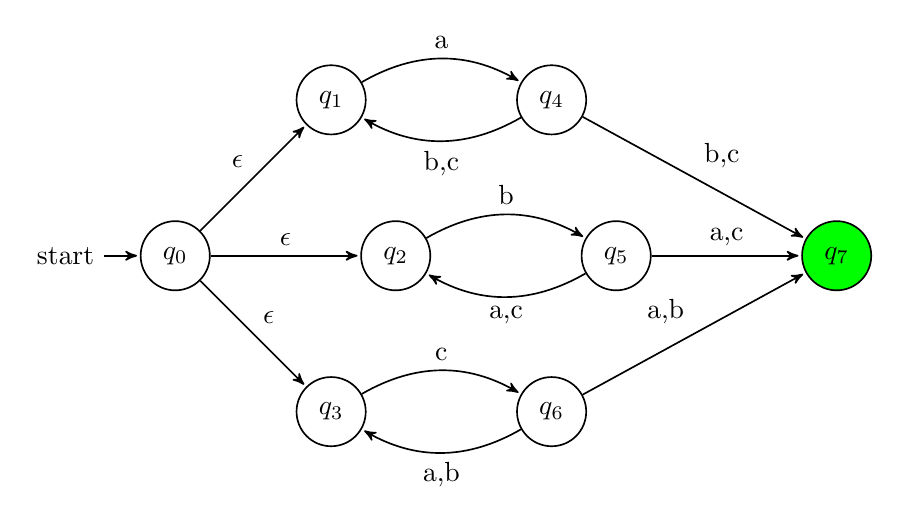
\begin{tikzpicture}[->,>=stealth',shorten >=1pt,auto,node distance=2.8cm,semithick]
  \tikzstyle{every state}=[fill=none,draw=black,text=black]

  \node[initial,state] (A)                    {$q_0$};
  \node[state]         (B) [above right of=A] 	  {$q_1$};
  \node[state]         (C) [right of=A] 	  {$q_2$};
  \node[state]         (F) [below right of=A] 	  {$q_3$};
  \node[state]         (G) [right of=B] 	  {$q_4$};
  \node[state]         (D) [right of=C]  {$q_5$};
  \node[state]		   (E) [right of=F] {$q_6$};
  \node[state]         (H) [right of=D,fill=green] 	  {$q_7$};

  \path (A) edge              node {$\epsilon$} (B)
  			edge              node {$\epsilon$} (C)
  			edge              node {$\epsilon$} (F) 
        (B) edge [bend left]  node {a} (G)
        (C) edge [bend left]  node {b} (D)
        (D) edge [bend left]  node {a,c} (C)
        	edge     	 	  node {a,c} (H)
        (E) edge [bend left]  node {a,b} (F)
        	edge     	 	  node {a,b} (H)
        (F) edge [bend left] node {c} (E)
        (G) edge [bend left]  node {b,c} (B)
            edge  	 	 	  node {b,c} (H);
\end{tikzpicture}


\end{document}